
\documentclass[12pt]{article}


\usepackage{epsfig}
\usepackage{amsmath,amsthm}
\usepackage{listings}
\usepackage{graphicx}
\graphicspath{ {./images/} }

\newtheorem{lemma}{Lemma}
\newtheorem{theorem}{Theorem}


\usepackage{titlesec}
\titleformat{\section}
{\normalfont\Large\bfseries}{Question~\thesection:}{1em}{}

\newlength{\toppush}
\setlength{\toppush}{2\headheight}
\addtolength{\toppush}{\headsep}


\def\subjnum{Comp 170}
\def\subjname{Computation Theory}


\def\doheading#1#2#3{\vfill\eject\vspace*{-\toppush}%
  \vbox{\hbox to\textwidth{{\bf} \subjnum: \subjname \hfil Erli Cai}%
    \hbox to\textwidth{{\bf} Tufts University, Fall 2020 \hfil#3\strut}%
    \hrule}}


\newcommand{\htitle}[1]{\vspace*{1.25ex plus 1ex minus 0ex}%
\begin{center}
{\large\bf #1}
\end{center}} 



\begin{document}
\setlength\parindent{0pt}
\doheading{2}{title}{Homework 01}


\section{}
We define $\hat{\delta}$ as  $\hat{\delta} : Q \times \Sigma^* \rightarrow Q$ inductively as:
\begin{equation}
 \hat{\delta} (q, \epsilon) = q \quad \mbox{for all }q \in Q
\end{equation}

\begin{equation}
\hat{\delta} (q, xa) = \delta(\hat{\delta}(q,x),a) \quad \mbox{for all }q \in Q, x \in \Sigma^*. a \in \Sigma
\end{equation}

\begin{flalign*}
a. \quad \hat{\delta}(p,a) &=  \hat{\delta}(p,\epsilon a)  &&\\
    & =  \delta(\hat{\delta}(p,\epsilon),a)  \quad \mbox{by definition (2)} \\
    & = \delta(p,a) \quad \mbox{by definition (1)}
\end{flalign*}


b.  We define $\delta_C$ to be the transition function for product construction such that\\
\begin{equation}
\delta_C((p,q),a) = (\delta_A(p,a),\delta_B(q,a)) \quad\mbox{for all a}\in\Sigma
\end{equation}

Let P(n) be the statement $\hat{\delta}_C((p,q),x) = (\hat{\delta}_A(p,x),\hat{\delta}_B(q,x)) \quad\mbox{for all }x\in\Sigma^* \mbox{ with length n }$. We want to show P(n) is true for all $ n \geq 0$\\

\textbf{Base case:} we want to show P(n) is true for n = 0\\
By definiton(1), we have
\begin{equation*}
\hat{\delta}_C((p,q),\epsilon) =(p,q) = (\hat{\delta}_A(p,\epsilon),\hat{\delta}_B(q,\epsilon))  \\
\end{equation*}
\textbf{Induction Hypothesis:} Assume P(n) is true for $n < k$, where k is a fixed integer, that is\\
$\hat{\delta}_C((p,q),x) = (\hat{\delta}_A(p,x),\hat{\delta}_B(q,x)) \quad\mbox{for all }x\in\Sigma^* \mbox{ with length less than k }$.

\pagebreak

\textbf{Induction Step:} we want to prove P(k), that is,\\
$\hat{\delta}_C((p,q),y) = (\hat{\delta}_A(p,y),\hat{\delta}_B(q,y)) \quad\mbox{for all }y\in\Sigma^* \mbox{ with length  k }$.
\begin{flalign*}
LHS &=  \hat{\delta}_C((p,q),y' a) \quad\mbox{where } y' \mbox{ has length k-1 }  &&\\
        &= \delta_C(\hat{\delta}_C((p,q),y'),a)  \quad\mbox{by definition(2)}\\
        &= \delta_C( (\hat{\delta}_A(p,y'),\hat{\delta}_B(q,y'))  ,a)  \quad\mbox{by induction hypothesis}\\
        &=  (\delta_A(\hat{\delta}_A(p,y'),a),\delta_B(\hat{\delta}_B(q,y'),a))   \quad\mbox{by definition(3)}\\
        &= (\hat{\delta}_A(p,y),(\hat{\delta}_A(p,y))\quad\mbox{ by definition (2)}\\
        &= RHS 
\end{flalign*}\\

By mathematical induction, we have P(n) is true for all $n\ge0$
\pagebreak


\section{}


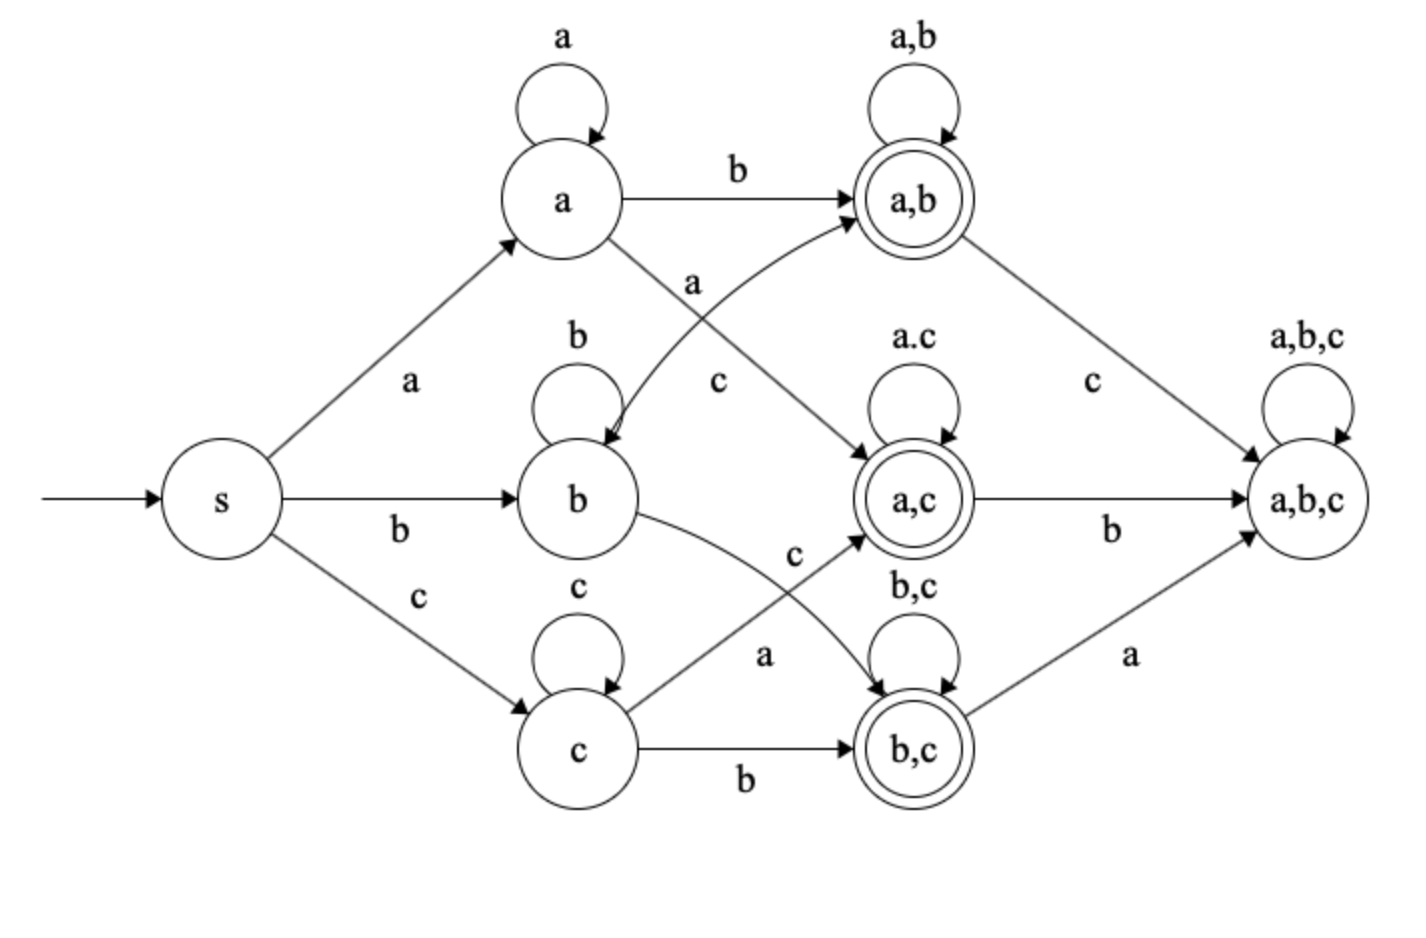
\includegraphics[width=\textwidth]{q2}
a. The character inside a node denote what characters have already appeared. The node where exactly two characters have appeared are accepted states.




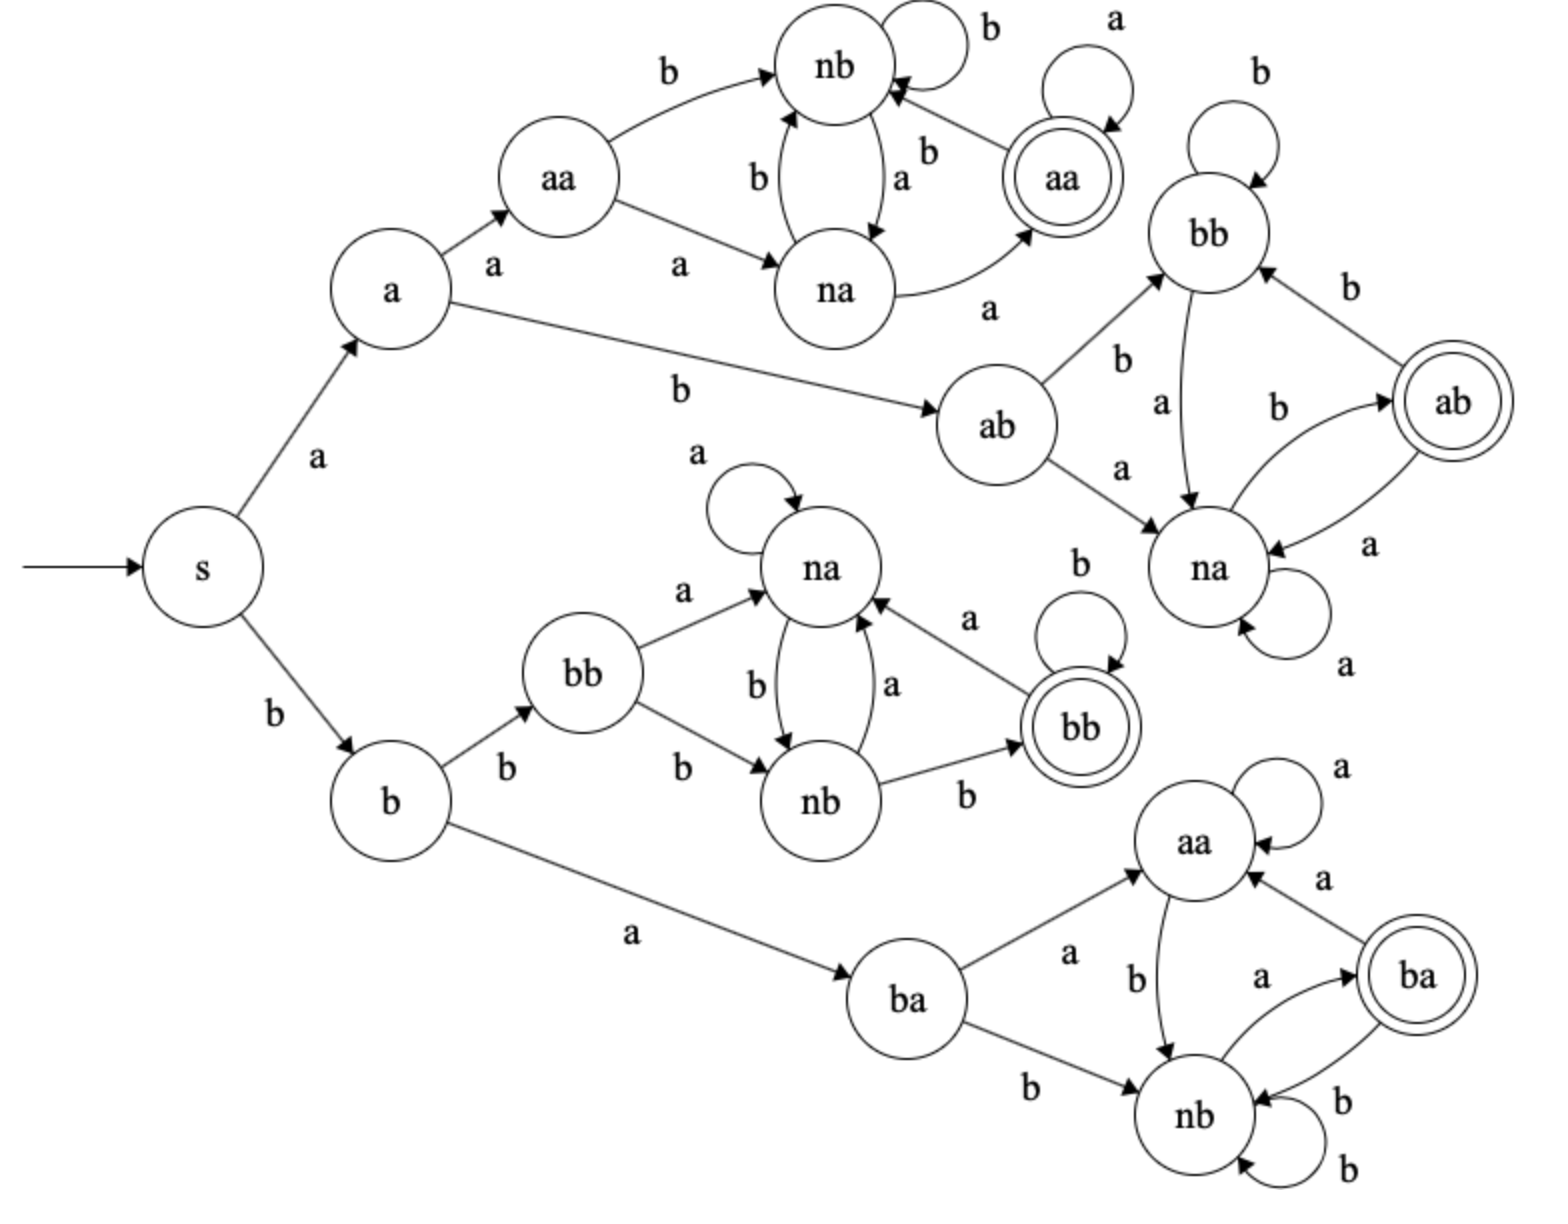
\includegraphics[width=\textwidth]{q3}
b. The characters in a node represent the last two characters in x(in same order) or last one character if x has length 1.  n means it could be either a or b. e.g. nb means it's either ab or bb.\\

From start state, it takes at least 4 steps to get to an accepted state. This ensures we won't accept string like aaa.\\

If you input aayaa, you will find you pass two different states denoted as aa(and you could do similar thing for ab, bb, ba as well). The first one denote the first two characters in x is aa. And the other one which is also an accepted state denote that the last two characters are aa.

\pagebreak


\section{}

Given a general DFA $M = (Q,\Sigma,\delta,s,F) $ accepting A, we define $M' =  (Q',\Sigma,\delta',s',F') $ where,
\begin{align*}
   Q' &= Q \cup Q \times \Sigma \cup \{d\}\\
   \delta'(p, a) &= (p, a) & \textrm{ for all $a \in \Sigma, p \in Q $ and $p\ne d$}\\
   \delta'(d, a) &= d & \textrm{ for all $a \in \Sigma$} \\
   \delta'((p, a), b) &= \begin{cases}
   \delta(p, a) &  \textrm{ if $p \in Q, b = a$}\\
   \ d  &\textrm{ if $p \in Q, b \ne a$}\\
   \end{cases}\\
   s' &= s&\\
   F' &= F
\end{align*}

M' has three types of state. First, it includes all the states of the original machine M and it also has states corresponding to state-character pairs. Other than that, it has a state corresponding to the strings not accepted by machine M'. When M' in a state $q \in Q\times\Sigma$, if it reads a character corresponds to the previous alphabet it will goes back to a state in Q. Otherwise, it will transition into state d, which indicates that the string is not accepted , and stays in state d forever.








\end{document}


